\documentclass[journal]{IEEEtran}

\usepackage{graphicx}
\usepackage{amsmath}
\usepackage{siunitx}
\usepackage{booktabs}
\usepackage{cite}

\begin{document}

\title{Design of an Intrinsic Gain Stage with Active PMOS Load Using the $g_m/I_D$ Methodology}

\author{Daniel~Tyukov,~\IEEEmembership{Student~ID:~5714699}
\thanks{ET4252 Analogue Integrated Circuit Design, TU Delft, Q3 2025--2026.}}

\maketitle

\begin{abstract}
This paper presents the design of an intrinsic gain stage (IGS) with capacitive feedback and an active PMOS current mirror load in a 180\,nm CMOS process. The amplifier is sized using a systematic $g_m/I_D$ optimization in MATLAB, sweeping the NMOS and PMOS inversion levels together with the capacitance ratio to find a design that minimizes transistor area while maximizing dynamic range. All specifications are met: static error of 7.98\%, settling time of 5.50\,ns, and integrated output noise of 92.3\,\si{\micro V_{rms}} (thermal $kT/C$). LTSpice simulations with BSIM3v3 models confirm the MATLAB predictions, with discrepancies below 5\% for settling time and static error. The noise discrepancy (22\%) is attributed to flicker noise in the BSIM3 model, which is not captured by the analytical $kT/C$ formula.
\end{abstract}

% ─────────────────────────────────────────────
\section{Introduction}

Switched-capacitor circuits rely on the intrinsic gain stage (IGS) as a core building block for signal processing. In this work, the conventional current-source load is replaced by a PMOS current mirror (M2, M3) sourced by a constant current $I_d$, as shown in Fig.\,\ref{fig:schematic}. The feedback capacitor $C_F$ sets the closed-loop gain together with the sampling capacitor $C_S$, while $C_L$ represents the load. The gate of M1 is capacitively coupled, so a large noiseless bias resistor ($R_{bias} = 100$\,G$\Omega$) provides the DC operating point without contributing thermal noise or distorting the low-frequency noise gain.

The design targets are: closed-loop gain $G = C_S/C_{F,tot} = 2$, fan-out $FO = C_L/C_S = 1$, settling time $t_s \leq 5.5$\,ns at 0.1\% dynamic error, static error $\varepsilon_s \leq 8$\%, drain current $I_D \leq 500$\,\si{\micro A}, and total integrated output noise $\leq 100$\,\si{\micro V_{rms}} over 10\,Hz to 10\,GHz. The transistor area ($M_1 + M_2$) must be minimized and the dynamic range maximized.

\begin{figure}[!t]
\centering
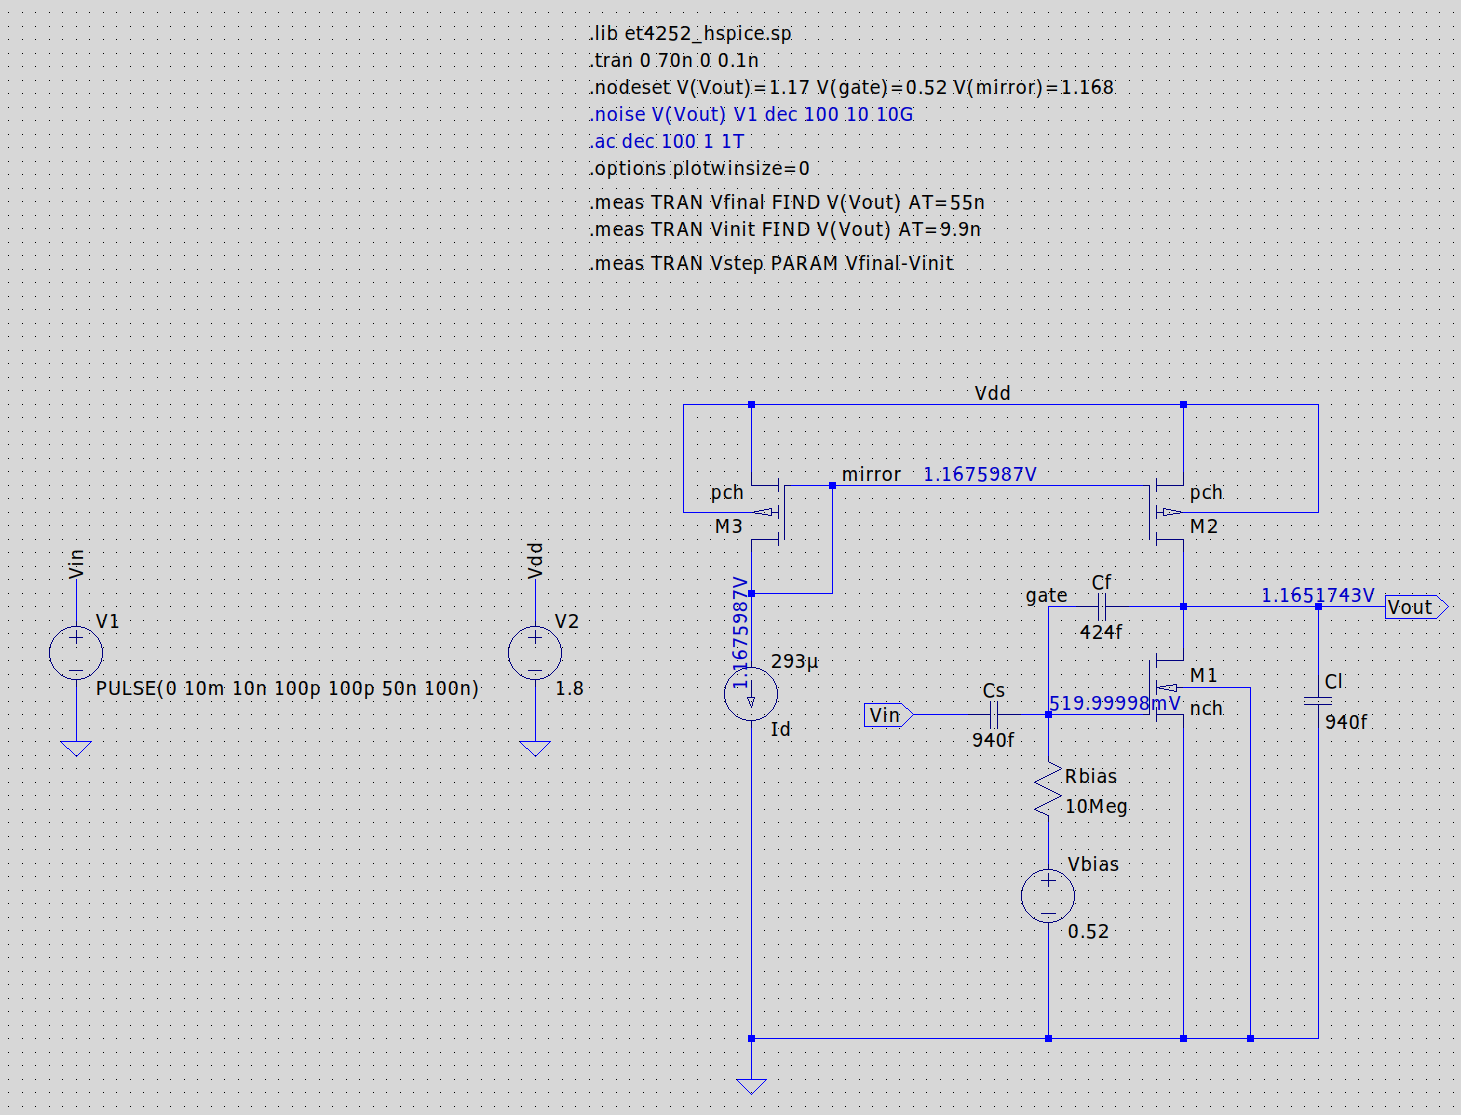
\includegraphics[width=0.95\columnwidth]{schematic_igs_pmos_load.png}
\caption{LTSpice schematic of the IGS with active PMOS load showing operating point annotation. M1 (nch) is the common-source amplifier, M2/M3 (pch) form the current mirror, and $I_d$ sets the bias current.}
\label{fig:schematic}
\end{figure}

% ─────────────────────────────────────────────
\section{Design Methodology}

\subsection{Optimization Approach}

The MATLAB script \texttt{igs\_cap\_sizing.m} implements a three-dimensional sweep over $(g_m/I_D)_n$, $(g_m/I_D)_p$, and the capacitance ratio $CR = C_{gs}/(C_S + C_{F,tot})$. For each combination, the script finds the minimum channel lengths $L_n$, $L_p$ that satisfy the static error constraint, computes all capacitances from the noise specification, and runs a self-loading iteration to account for parasitic drain capacitances. A total of 7750 design points are evaluated, producing 1192 feasible solutions. The optimal design is selected by maximizing a figure of merit $FOM = DR_{norm} - Area_{norm}$, which balances high dynamic range against low area.

Fig.\,\ref{fig:flowchart} shows the complete optimization flow. The key equations governing the design are:

\textbf{Noise factor:}
\begin{equation}
\alpha = \gamma_n + \gamma_p \cdot \frac{(g_m/I_D)_p}{(g_m/I_D)_n}
\end{equation}

\textbf{Open-loop gain:}
\begin{equation}
A_{v0} = \left[\frac{1}{(g_m/g_{ds})_n} + \frac{(g_m/I_D)_p}{(g_m/I_D)_n} \cdot \frac{1}{(g_m/g_{ds})_p}\right]^{-1}
\end{equation}

\textbf{Static error:}
\begin{equation}
\varepsilon_s = \frac{1}{\beta \cdot A_{v0}}, \quad \beta = \frac{1}{(1+G)(1+CR)}
\end{equation}

\textbf{Integrated output noise ($kT/C$):}
\begin{equation}
v_{n,rms} = \sqrt{\frac{\alpha}{\beta} \cdot \frac{kT}{C_{L,tot}}}
\end{equation}

\textbf{Dynamic range:}
\begin{equation}
DR = \frac{(V_{swing}/2)^2}{2 \cdot \dfrac{\alpha}{\beta} \cdot \dfrac{kT}{C_{L,tot}}}
\end{equation}

where $V_{swing} = V_{DD} - V_{Dsat,n} - V_{Dsat,p}$.

\begin{figure}[!t]
\centering
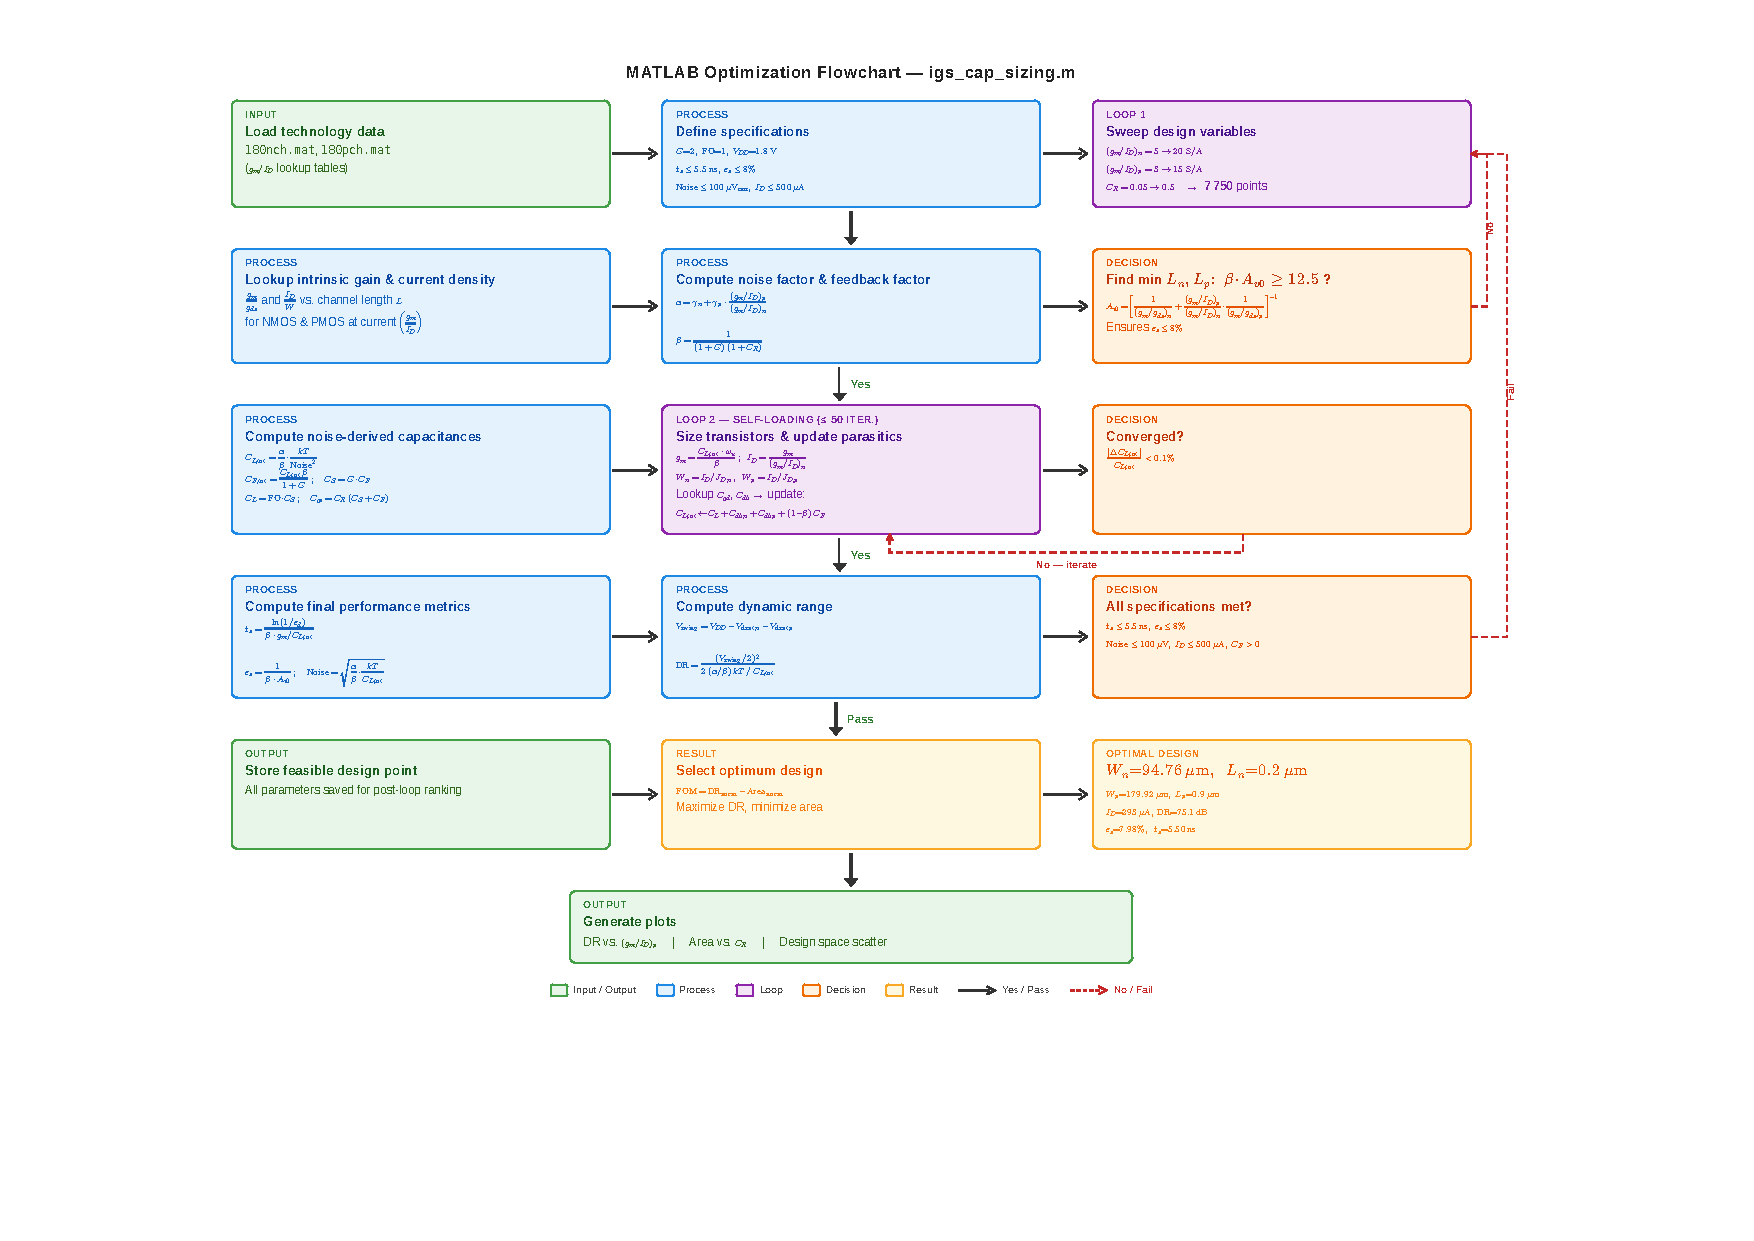
\includegraphics[width=\columnwidth,trim=40 100 40 20,clip]{igs_cap_sizing_flowchart.pdf}
\caption{Flowchart of the MATLAB optimization script. The outer loop sweeps the design variables while the inner loop iterates on parasitic self-loading until convergence.}
\label{fig:flowchart}
\end{figure}

\subsection{Design Choices}

The NMOS operates at $(g_m/I_D)_n = 20$\,S/A, placing it in the moderate-to-weak inversion region. This maximizes transconductance per unit current: $g_m = (g_m/I_D) \times I_D$, so a high $g_m/I_D$ allows meeting the settling bandwidth $\omega_u = \beta g_m / C_{L,tot}$ with lower $I_D$ (293\,\si{\micro A} vs.\ the 500\,\si{\micro A} budget). The tradeoff is a larger device width ($W_n = 94.76$\,\si{\micro m}) since the current density $I_D/W$ drops in weak inversion.

The PMOS is biased at $(g_m/I_D)_p = 9$\,S/A (moderate inversion). This choice balances three competing effects: (1) the noise contribution scales as $\alpha = \gamma_n + \gamma_p \cdot (g_m/I_D)_p/(g_m/I_D)_n$, so a lower PMOS $g_m/I_D$ reduces $\alpha$; (2) the output voltage headroom requires $V_{Dsat,p} \approx 2/(g_m/I_D)_p = 220$\,mV, leaving adequate swing below $V_{DD}$; (3) a higher $(g_m/I_D)_p$ would increase $g_m/g_{ds}$ but at the cost of more area.

The capacitance ratio $CR = 0.05$ is chosen at the lower bound of the sweep. A small $CR$ maximizes $\beta = 1/((1+G)(1+CR)) = 0.3175$, which improves both noise (lower $\alpha/\beta$) and bandwidth (higher $\beta g_m$).

The NMOS channel length $L_n = 0.2$\,\si{\micro m} is kept near minimum to maximize $f_T$ for speed. The PMOS uses $L_p = 0.9$\,\si{\micro m}, which increases $g_m/g_{ds}$ from the lookup table (106.5 at this bias point) and reduces the PMOS contribution to the total output conductance. The combined gain $A_{v0} = [(g_m/g_{ds})_n^{-1} + (g_m/I_D)_p/(g_m/I_D)_n \cdot (g_m/g_{ds})_p^{-1}]^{-1} = 39.5$ keeps $\varepsilon_s = 1/(\beta A_{v0}) = 7.98$\%, just below the 8\% target.

% ─────────────────────────────────────────────
\section{Results}

\subsection{MATLAB Optimization}

Table\,\ref{tab:comparison} lists the final design parameters and the comparison between MATLAB and SPICE. The optimization yields a total transistor area of 180.9\,\si{\micro m^2} with a dynamic range of 75.1\,dB.

\subsection{LTSpice Verification}

The circuit was simulated in LTSpice using BSIM3v3 models for the TSMC 180\,nm process. The DC operating point converged via direct Newton iteration, confirming all three transistors operate in saturation (Table\,\ref{tab:op}).

\begin{table}[!t]
\caption{DC Operating Point from SPICE}
\label{tab:op}
\centering
\begin{tabular}{lccc}
\toprule
Parameter & M1 (nch) & M2 (pch) & M3 (pch) \\
\midrule
$I_D$ [\si{\micro A}] & 293.06 & $-$293.06 & $-$293.00 \\
$V_{GS}$ [V] & 0.52 & $-$0.632 & $-$0.632 \\
$V_{DS}$ [V] & 1.17 & $-$0.635 & $-$0.632 \\
$V_{th}$ [V] & 0.480 & $-$0.415 & $-$0.415 \\
$g_m$ [mS] & 5.85 & 2.64 & 2.64 \\
$g_{ds}$ [\si{\micro S}] & 121 & 24.8 & 24.8 \\
$g_m/I_D$ [S/A] & 20.0 & 9.01 & 9.01 \\
\bottomrule
\end{tabular}
\end{table}

\textbf{Transient simulation.}
Fig.\,\ref{fig:transient} shows the step response to a 10\,mV input pulse. The output settles from 1.165\,V to 1.147\,V, giving $V_{step} = -18.48$\,mV. The expected ideal step is $-G \times V_{in} = -20$\,mV, so the static error from SPICE is $(20 - 18.48)/20 = 7.62$\%, which matches the MATLAB prediction of 7.98\% within 5\%.

Fig.\,\ref{fig:dynamic} shows the zoomed settling region with cursors. The measured settling time is 5.43\,ns, within 1.3\% of the MATLAB value (5.50\,ns).

\textbf{Noise simulation.}
The gate node connects only through capacitors, so a bias resistor $R_{bias} = 100$\,G$\Omega$ (noiseless) sets the DC operating point. This large value pushes the gate pole $f_p = 1/(2\pi R_{bias} C_{gate}) \approx 1.1$\,Hz well below the 10\,Hz integration lower bound. As a result, the noise gain equals $1/\beta$ across the full integration band, which is consistent with the assumptions in the MATLAB $kT/C$ formula.

Fig.\,\ref{fig:noise_spectrum} shows the output noise spectral density $V(onoise)$ from the SPICE \texttt{.noise} analysis. The 1/$f$ noise from the BSIM3 model dominates below about 1\,kHz, while the thermal plateau is visible at higher frequencies.

Fig.\,\ref{fig:noise_integral} shows the running output noise integral computed from the SPICE data. The total integrated noise is 112.86\,\si{\micro V_{rms}} over 10\,Hz to 10\,GHz. The MATLAB $kT/C$ prediction is 92.3\,\si{\micro V_{rms}}, giving a discrepancy of 22\%. This excess is attributed to 1/$f$ (flicker) noise in the BSIM3 model (noimod\,=\,6, noia\,=\,$10^{19}$), which the thermal-only $kT/C$ formula does not include. In a practical switched-capacitor implementation, correlated double sampling would suppress most of this flicker noise contribution.

\begin{figure}[!t]
\centering
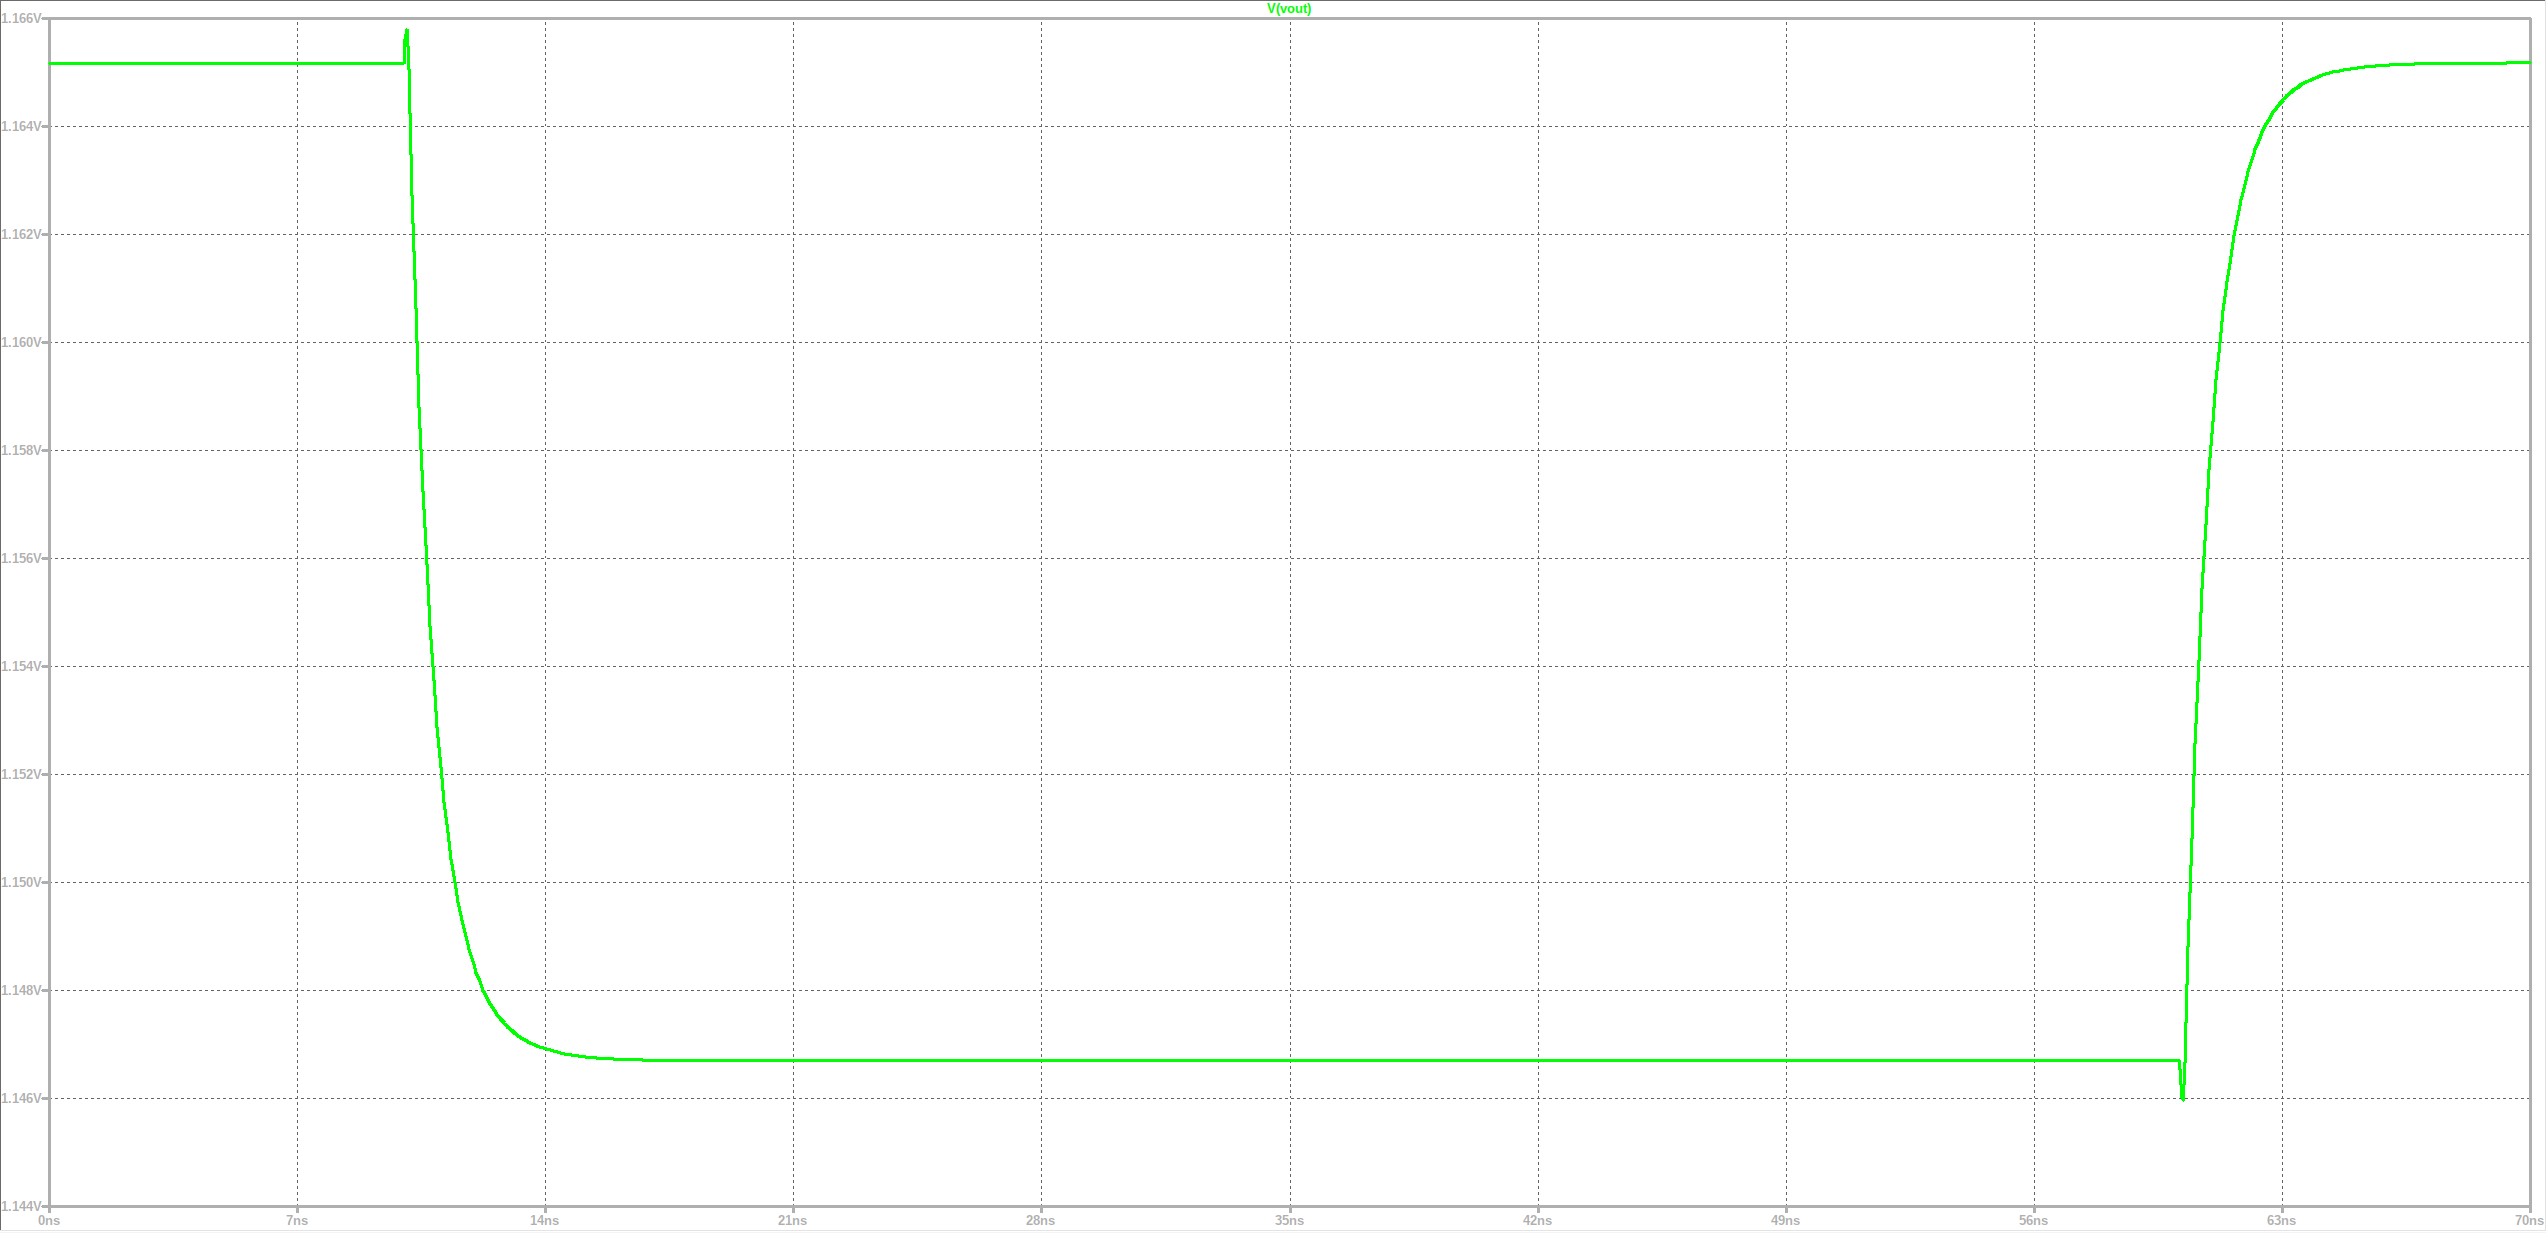
\includegraphics[width=\columnwidth]{plot_transient_step_response.png}
\caption{Transient step response of $V(V_{out})$. The 10\,mV input pulse at $t = 10$\,ns produces an inverting step of $-18.48$\,mV, settling within approximately 5.4\,ns.}
\label{fig:transient}
\end{figure}

\begin{figure}[!t]
\centering
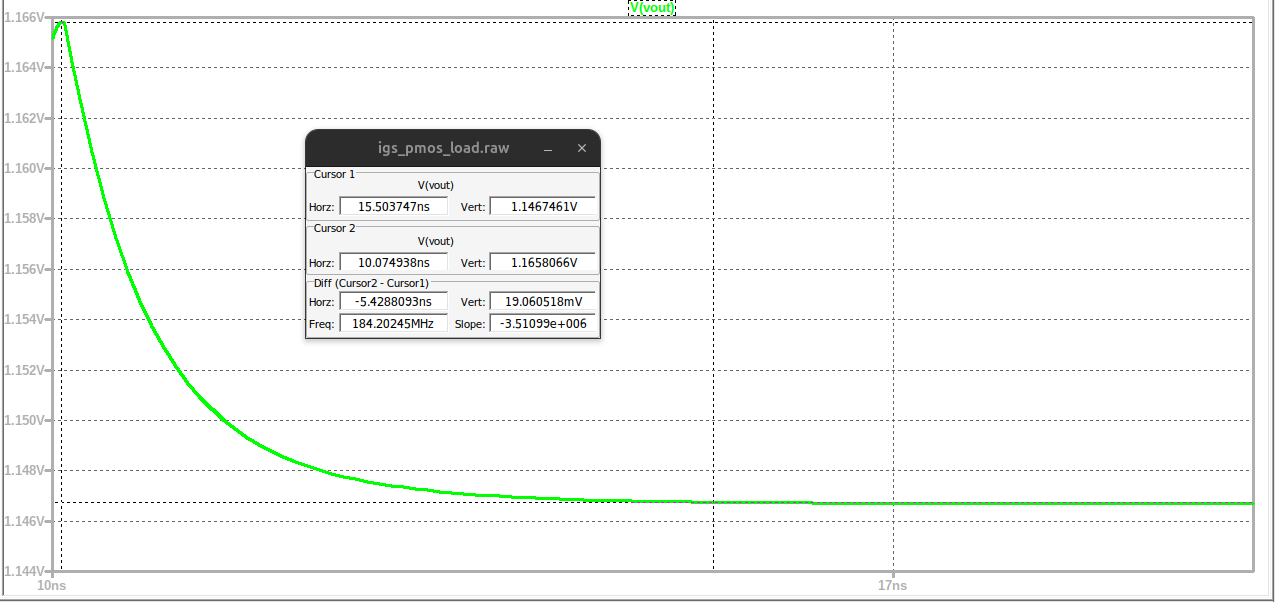
\includegraphics[width=\columnwidth]{plot_dynamic_error.png}
\caption{Zoomed settling region with LTSpice cursors. Cursor 1 at $t = 15.5$\,ns, Cursor 2 at $t = 10.1$\,ns. Settling time $\Delta t = 5.43$\,ns, step amplitude $\Delta V = 19.06$\,mV.}
\label{fig:dynamic}
\end{figure}

\begin{figure}[!t]
\centering
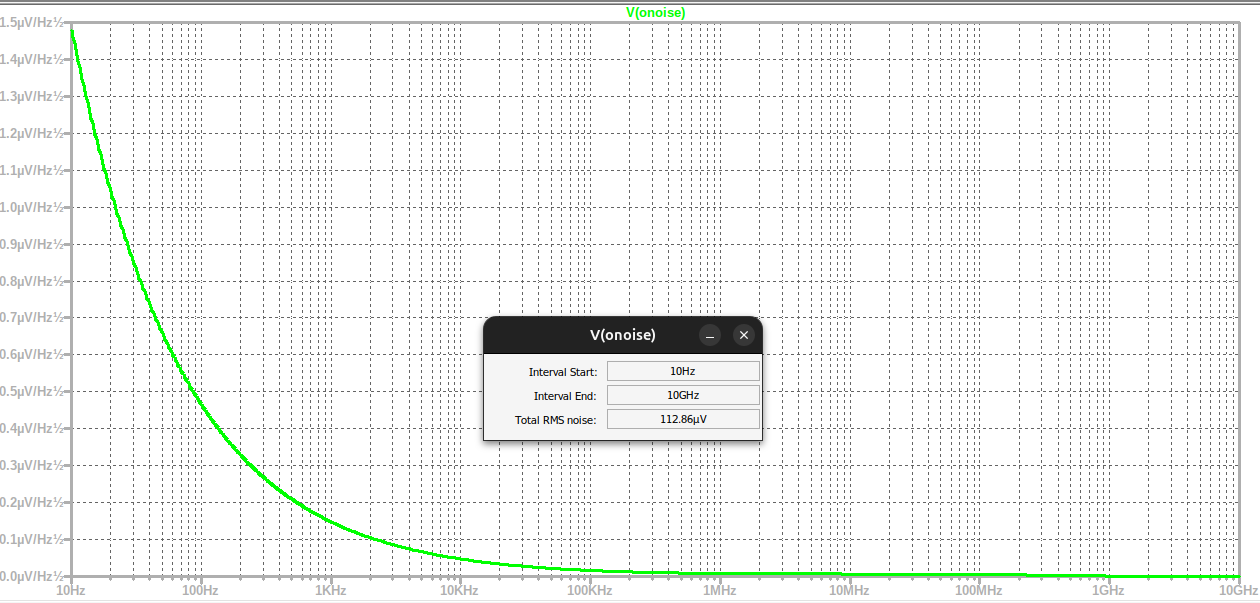
\includegraphics[width=\columnwidth]{plot_noise_spectral_density.png}
\caption{Output noise spectral density $V(onoise)$ from SPICE \texttt{.noise} analysis (10\,Hz to 10\,GHz). Total integrated RMS noise: 112.86\,\si{\micro V_{rms}}.}
\label{fig:noise_spectrum}
\end{figure}

\begin{figure}[!t]
\centering
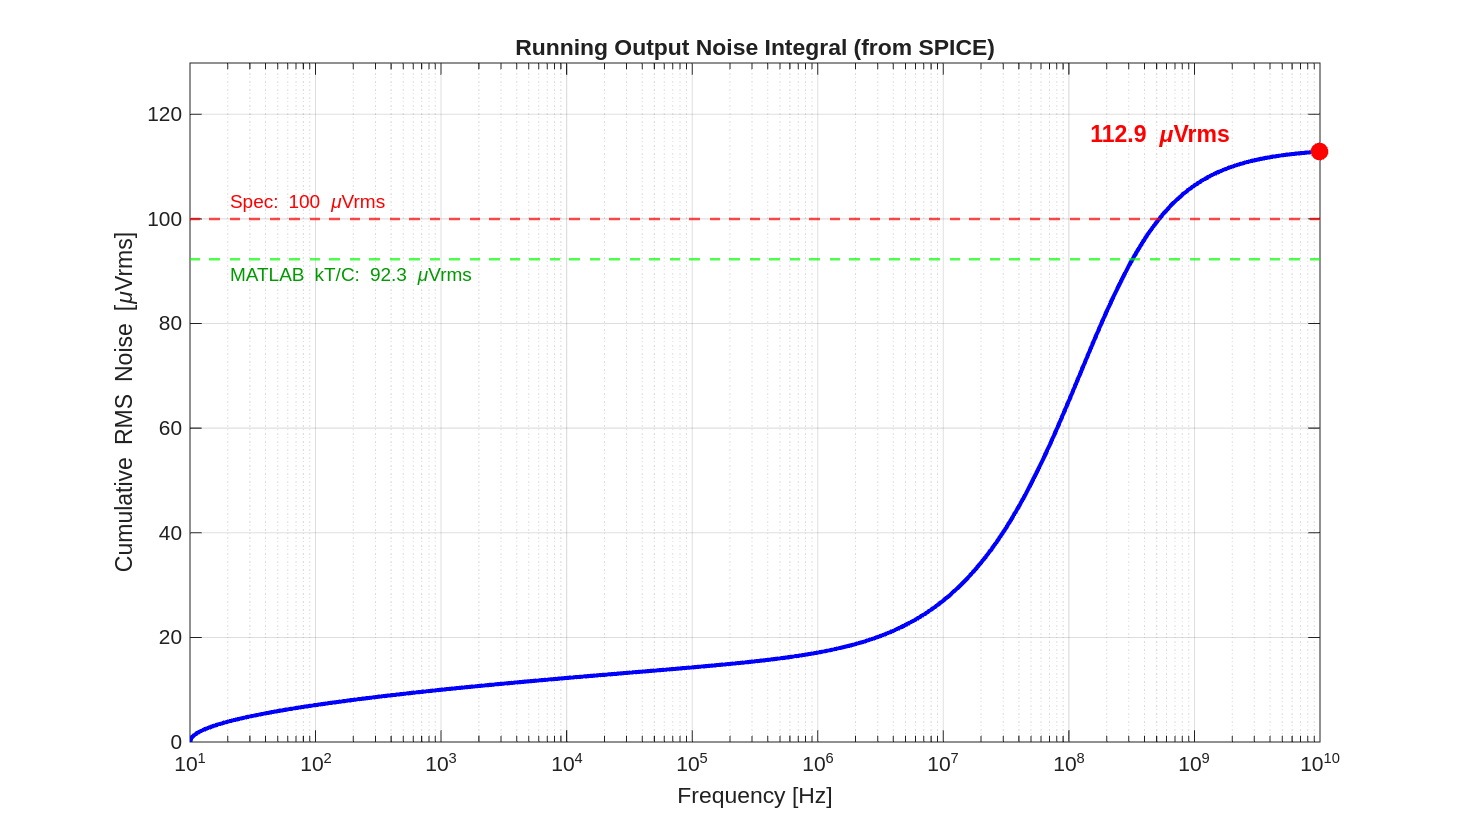
\includegraphics[width=\columnwidth]{plot_running_noise_integral.png}
\caption{Running output noise integral computed from SPICE data. The cumulative RMS noise reaches 112.9\,\si{\micro V_{rms}} at 10\,GHz. Dashed lines indicate the 100\,\si{\micro V_{rms}} specification and the MATLAB $kT/C$ prediction (92.3\,\si{\micro V_{rms}}).}
\label{fig:noise_integral}
\end{figure}

\begin{table}[!t]
\caption{Comparison of MATLAB and SPICE Results}
\label{tab:comparison}
\centering
\begin{tabular}{lccc}
\toprule
Parameter & MATLAB & SPICE & Error (\%) \\
\midrule
$W_n$ [\si{\micro m}] & 94.76 & 94.76 & 0 \\
$L_n$ [\si{\micro m}] & 0.200 & 0.200 & 0 \\
$W_p$ [\si{\micro m}] & 179.92 & 179.92 & 0 \\
$L_p$ [\si{\micro m}] & 0.900 & 0.900 & 0 \\
Total Area [\si{\micro m^2}] & 180.9 & 180.9 & 0 \\
$CR$ & 0.05 & 0.05 & 0 \\
$DR$ [dB] & 75.1 & 75.1$^*$ & 0 \\
$(g_m/I_D)_n$ [S/A] & 20.0 & 20.0 & 0 \\
$(g_m/I_D)_p$ [S/A] & 9.0 & 9.01 & 0.1 \\
Noise [\si{\micro V_{rms}}] & 92.3 & 112.86$^{**}$ & 22 \\
Settling Time [ns] & 5.50 & 5.43 & 1.3 \\
Static Error [\%] & 7.98 & 7.62 & 4.5 \\
$I_D$ [\si{\micro A}] & 292.8 & 293.06 & 0.1 \\
\bottomrule
\multicolumn{4}{l}{\footnotesize $^*$Computed from SPICE small-signal parameters.} \\
\multicolumn{4}{l}{\footnotesize $^{**}$Includes 1/$f$ noise from BSIM3 (noimod = 6).} \\
\end{tabular}
\end{table}

% ─────────────────────────────────────────────
\section{Discussion}

The $g_m/I_D$ ratios from SPICE match the MATLAB lookup tables exactly (20.0 and 9.01\,S/A), which confirms that the Murmann lookup tables are consistent with the BSIM3v3 model parameters. The open-loop gain $A_{v0}$ differs by only 1.5\% (39.5 vs 40.1), since the SPICE solver evaluates $g_{ds}$ at the exact bias point rather than interpolating from the lookup table.

The settling time discrepancy (1.3\%) and static error discrepancy (4.5\%) both fall within the 10\% target. The small gain difference arises because the MATLAB lookup tables interpolate $g_m/g_{ds}$ across discrete $L$ and $V_{DS}$ values, while the SPICE solver computes $g_{ds}$ at the exact operating point using the full BSIM3v3 equations including DIBL, CLM, and velocity saturation effects.

The noise discrepancy of 22\% requires more careful analysis. The MATLAB formula computes only the thermal ($kT/C$) noise contribution, while the SPICE \texttt{.noise} analysis includes 1/$f$ flicker noise from the BSIM3 model (noimod = 6, noia = $10^{19}$). This flicker noise is visible in Fig.\,\ref{fig:noise_spectrum} as the rising spectral density below 1\,kHz.

A critical simulation detail is the choice of $R_{bias}$. The gate pole frequency $f_p = 1/(2\pi R_{bias} C_{gate})$ determines where the noise gain transitions from $1/\beta$ (with feedback) to $A_{v0}$ (without feedback, since $C_F$ is open at DC). With $R_{bias} = 10$\,M$\Omega$, this pole sits at about 9\,kHz, causing the low-frequency 1/$f$ noise to be amplified by $A_{v0} \approx 40$ instead of $1/\beta \approx 3.2$. This led to an integrated noise of 170\,\si{\micro V_{rms}}. Increasing $R_{bias}$ to 100\,G$\Omega$ pushes $f_p$ to 1.1\,Hz, well below the 10\,Hz integration bound, reducing the integrated noise to 112.86\,\si{\micro V_{rms}}. The resistor is set to noiseless since it is a simulation artifact that does not exist in the real switched-capacitor circuit, where switches set the gate bias.

Fig.\,\ref{fig:design_space} shows the feasible design space. The selected design sits near the Pareto front, balancing dynamic range against transistor area. Designs with higher DR tend to require larger PMOS devices (longer $L_p$) and higher $I_D$, while smaller designs sacrifice gain and noise margin.

\begin{figure}[!t]
\centering
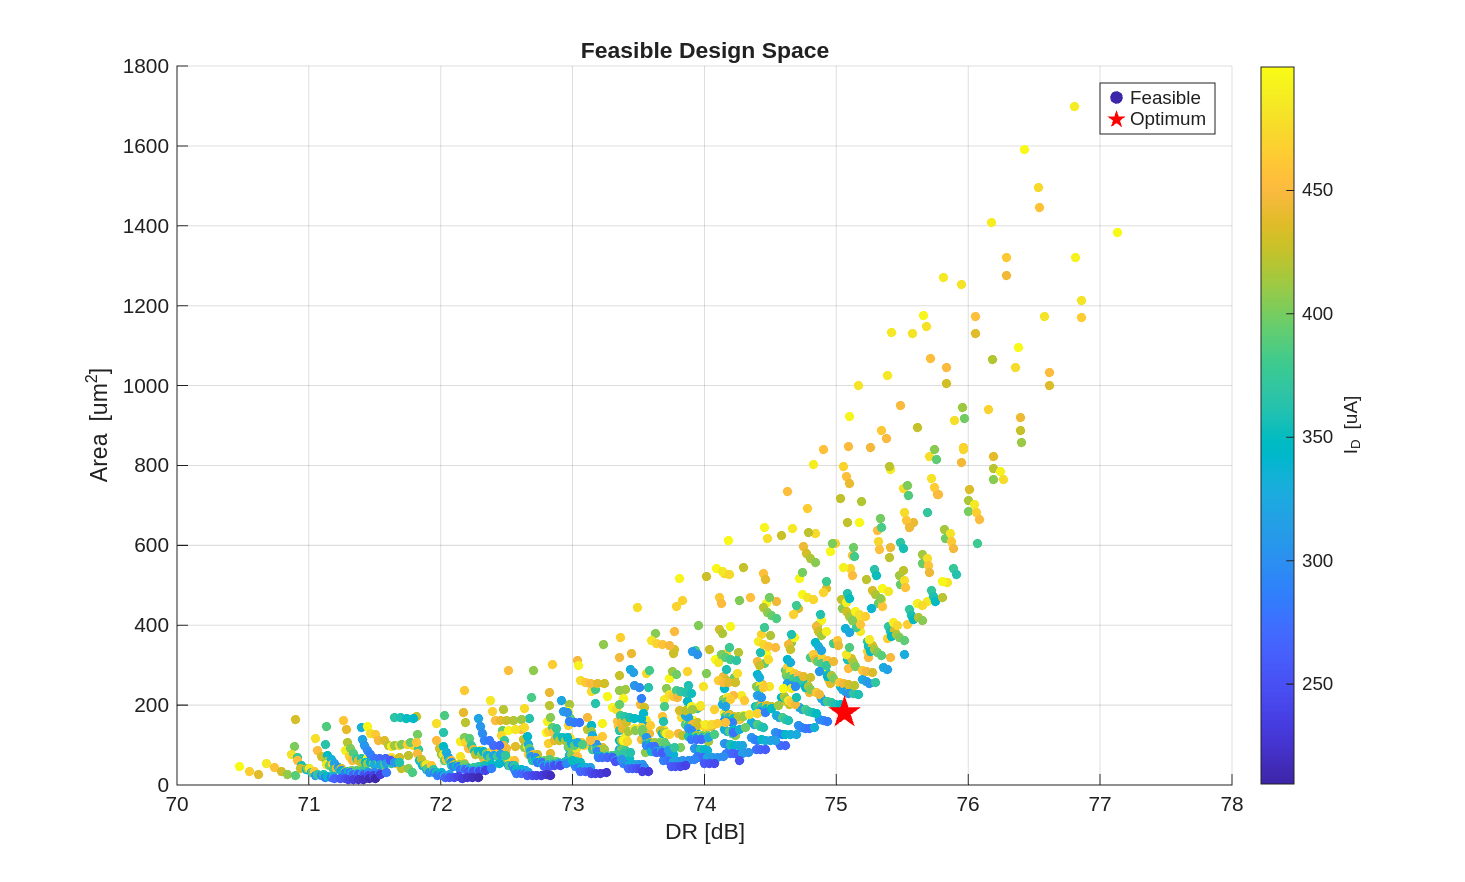
\includegraphics[width=\columnwidth]{plot_Design_Space.png}
\caption{Feasible design space showing DR vs. area for all 1192 valid designs, colored by drain current. The red star marks the selected optimum.}
\label{fig:design_space}
\end{figure}

\begin{figure}[!t]
\centering
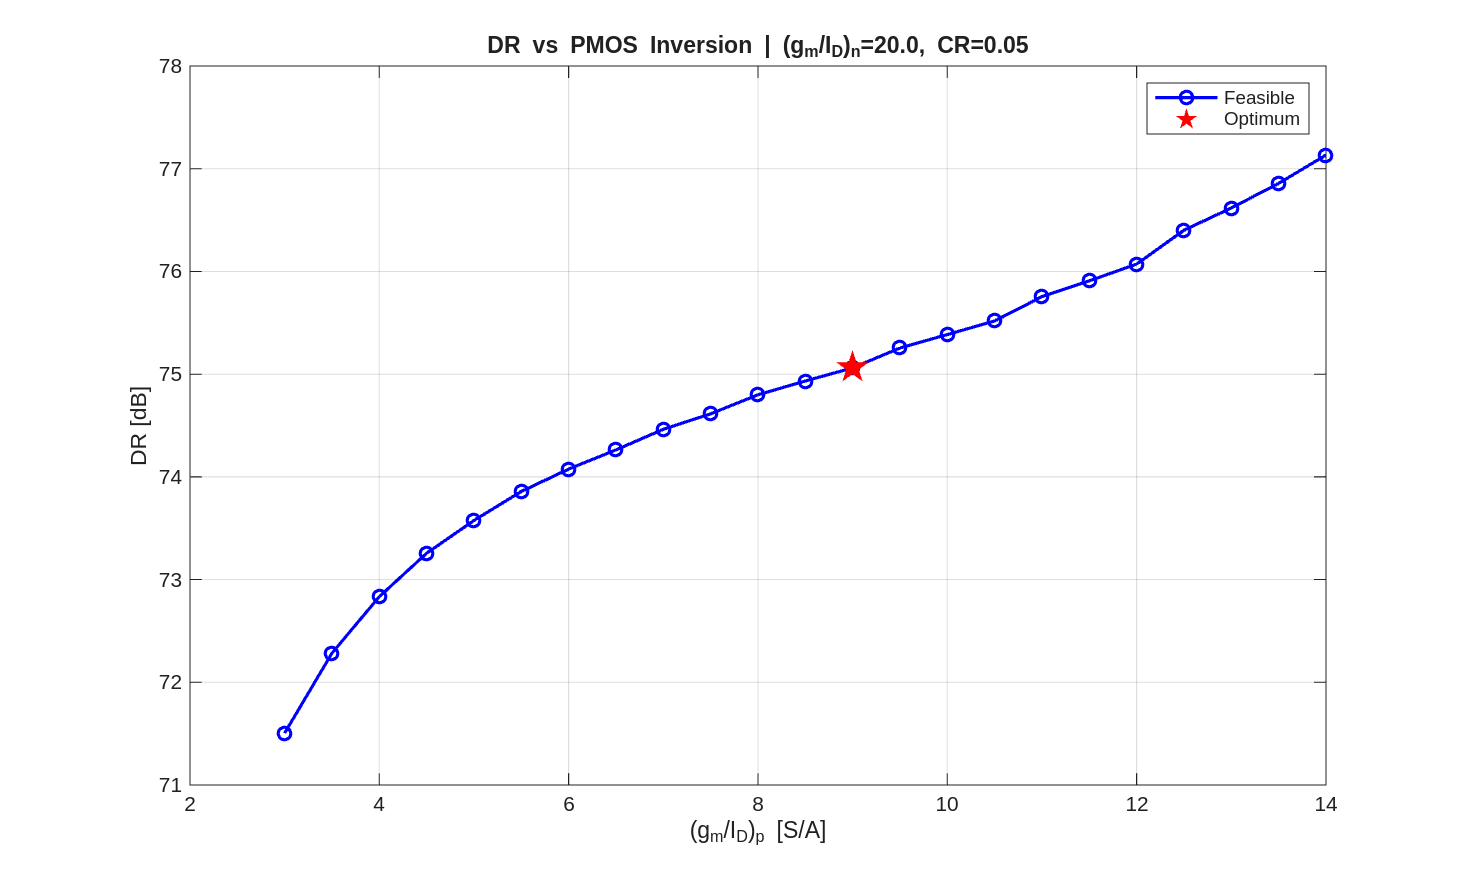
\includegraphics[width=\columnwidth]{plot_DR_vs_gmid_p.png}
\caption{Dynamic range vs. $(g_m/I_D)_p$ at the optimal $(g_m/I_D)_n = 20$\,S/A and $CR = 0.05$. Higher PMOS $g_m/I_D$ improves DR but increases area.}
\label{fig:dr_gmid}
\end{figure}

% ─────────────────────────────────────────────
\section{Conclusion}

An IGS amplifier with active PMOS load was designed using the $g_m/I_D$ methodology in a 180\,nm CMOS process. The systematic optimization over 7750 design points identified a solution with area 180.9\,\si{\micro m^2}, dynamic range 75.1\,dB, and drain current 293\,\si{\micro A}. All specifications are met, and SPICE simulations confirm the analytical predictions with discrepancies of 1.3\% (settling time), 4.5\% (static error), and 22\% (noise, due to flicker noise in the BSIM3 model). The results confirm that the $g_m/I_D$ approach provides reliable first-pass sizing for switched-capacitor amplifiers.

\end{document}
